\documentclass[11pt,a4paper]{article}
\usepackage{fontspec}
\setmainfont{TeX Gyre Pagella}
\usepackage[a4paper,margin=2.4cm]{geometry}
\usepackage{amsmath}
\usepackage{graphicx,booktabs,float,caption,array,xcolor,longtable}
\usepackage{xurl}
\usepackage[hidelinks]{hyperref}
\usepackage{titlesec}
\usepackage[round,authoryear]{natbib}
\usepackage{setspace}
\setstretch{1.08}
\renewcommand{\topfraction}{0.9}
\renewcommand{\bottomfraction}{0.8}
\renewcommand{\textfraction}{0.1}
\renewcommand{\floatpagefraction}{0.75}
\setlength{\parindent}{0pt}
\setlength{\parskip}{0.55em}
\titleformat{\section}{\bfseries\Large}{\thesection}{0.8em}{}
\titleformat{\subsection}{\bfseries\large}{\thesubsection}{0.8em}{}
\captionsetup{font=small,labelfont=bf}
\urlstyle{same}
\hypersetup{pdftitle={Does Rain Keep Britain at Home?},pdfauthor={Tristan Hotham}}

\begin{document}
\begin{center}
{\LARGE\bfseries Does Rain Keep Britain at Home?\par}
\vspace{0.4em}
{\large Polling-day weather, turnout and party support at UK general elections, 1945 to 2024\par}
\vspace{1.2em}
{\large Dr Tristan Hotham\par}
\vspace{0.3em}
{\small Independent researcher\\
ORCID: 0000-0003-4931-9349\\
DOI: https://doi.org/10.5281/zenodo.24094534\par}
\vspace{0.8em}
2026
\end{center}

\begin{quote}
\small
\begin{center}\textbf{Abstract}\end{center}
Rain on polling day is widely believed to depress turnout and, in some accounts, to help parties of the right. Evidence, with mixed results, comes mostly from the United States and a few European countries; Britain has had little systematic study. I match each of the 14{,}052 contested constituency contests at the 22 UK general elections from 1945 to 2024 to hourly ERA5 reanalysis precipitation at the seat's grid cell during that election's actual polling hours, and test hypotheses set out in a written plan before estimation. With seat and election fixed effects, each centimetre of polling-hours rain is associated with turnout 0.96 percentage points lower (95\% CI -1.82 to -0.11; standard errors clustered by seat and by election and region). The sign is stable across alternative fixed effects, measures of rain and leave-one-out samples. But inference that respects the small number of elections is less favourable: a wild cluster bootstrap by election gives $p=0.14$, and randomisation inference that swaps whole national rain maps between elections gives $p=0.10$. Rain on the day before polling day, a placebo, shows an association of similar size that is at least as unusual under the same inference. Rain has no detectable association with Conservative or Labour vote shares, and, contrary to expectation, the turnout association is not weaker after postal voting on demand was introduced in 2001. The data rule out large effects of rain on British turnout, but cannot establish that rain lowers it at all.

\textbf{Keywords:} turnout; weather; rainfall; cost of voting; British general elections; randomisation inference; ERA5
\end{quote}

\section{Introduction}
Few pieces of electoral folklore are as durable as the idea that bad weather keeps voters at home. Party workers watch the forecast on polling day, commentators reach for the weather when turnout disappoints, and in the United States the claim that ``the Republicans should pray for rain'' has become a staple of both political science and popular writing \citep{gomez2007}. The logic is simple. Voting has costs, and anything that raises them on the day should, at the margin, reduce the number of people who vote \citep{downs1957,rikerordeshook1968}. Rain is an unusually attractive source of such costs for researchers because it is plausibly unrelated to the political characteristics of a place in a given year: it falls on safe seats and marginal ones, on rich and poor areas, regardless of the campaign.

The empirical record, however, is less settled than the folklore. Large studies of US presidential elections find that rain lowers turnout by around one percentage point per inch \citep{gomez2007} and use the variation to study partisan consequences \citep{hansfordgomez2010} or habit formation \citep{fujiwara2016}. Studies in the Netherlands \citep{eisinga2012turnout} and Denmark \citep{damsbo2023} also find that rain lowers turnout, by between about 0.4 and 1 point per centimetre; studies in Sweden find no robust effect \citep{persson2014}; and a study of Norwegian municipalities finds that rain \emph{raised} turnout \citep{lind2020}. Methodological work has shown that conventional standard errors understate the uncertainty in rainfall designs, because rain is spatially correlated within an election \citep{cooperman2017}, and that weather affects so many things that its use as an instrument is fraught \citep{mellon2025}.

Britain is a natural but neglected case. Its general elections are held on a single day, in a single country with a famously changeable climate, under single-member districts whose turnout is recorded seat by seat back to the nineteenth century. Yet, to my knowledge, no study has related polling-day weather to turnout across the full post-war sequence of UK general elections. This paper does so. I match the 14{,}052 contested constituency contests at the 22 general elections from 1945 to 2024 to hourly precipitation and temperature from the ERA5 reanalysis \citep{hersbach2020}, summed over each election's actual polling hours, and estimate the association between rain and turnout within seats, net of each election's national level. I also ask whether rain shifts party shares and whether the introduction of postal voting on demand in 2001 changed the relationship.

The answer is deliberately cautious. The planned main estimate is negative, close in size to the Danish estimate per centimetre, and its sign survives every alternative specification. But it rests on 22 elections, and when inference respects that fact the evidence is weak. A placebo using the previous day's rain produces a coefficient of similar size, and one that is at least as unusual under the same few-cluster inference, which suggests either that weather around polling day matters through channels other than the cost of getting to the polling station, or that some residual spatial confounding remains. I find no partisan effect. The contribution is therefore twofold: a long-run British estimate that bounds the plausible effect of rain on turnout to small values, and a demonstration, with randomisation inference built from real weather maps, of how much uncertainty a rainfall design carries when the number of independent weather draws is small.

The paper proceeds as follows. Section~\ref{sec:lit} reviews the literature. Section~\ref{sec:data} describes the data, Section~\ref{sec:design} the design, and Section~\ref{sec:results} the results. Section~\ref{sec:rob} reports robustness checks and placebos, Section~\ref{sec:disc} discusses the findings and their limits, and Section~\ref{sec:concl} concludes.

\section{Background and literature}\label{sec:lit}
\subsection{Weather as a cost of voting}
The calculus of voting treats the decision to vote as a comparison of costs with the expected benefits and the satisfaction of doing one's duty \citep{downs1957,rikerordeshook1968}. Because the probability of being pivotal in a large electorate is tiny, small changes in costs can matter for citizens near the margin of indifference. Reviews of aggregate turnout research list weather among the situational factors that can shift turnout, alongside closeness, electoral rules and the costs of registration and voting \citep{geys2006,blais2006}. Weather is attractive to researchers not because it is an important cause of turnout overall, but because it varies in a way that is plausibly unrelated to voters' preferences.

\citet{gomez2007} gave the modern statement of the argument. Using county-level returns from fourteen US presidential elections and data from more than 22,000 weather stations, they found that each inch of rain above normal reduced turnout by just under one percentage point, with snow having a smaller effect, and that bad weather benefited Republican candidates. \citet{knack1994}, using survey data from the 1980s, had found no general effect of rain on the probability of voting, except among respondents with a weak sense of civic duty. \citet{fragahersh2010} showed that the US effect of rain was concentrated in uncompetitive contests and disappeared in competitive ones, an early indication that the effect is conditional on context.

\subsection{Evidence beyond the United States}
Outside the United States, results vary. \citet{eisinga2012turnout} matched 13 Dutch parliamentary elections from 1971 to 2010 to weather at the nearest station for more than 400 municipalities and found that about 25 mm of rain lowered turnout by about one percentage point, while warmer and sunnier days raised it. \citet{persson2014} examined Swedish elections with municipal aggregates, election study surveys and register-based turnout and found no robust negative effect of rain in any of the three datasets; they argue that convenient voting, including early voting, may insulate turnout from weather. \citet{artes2014} found that rain lowered turnout in Spanish general elections. \citet{stockemerwigginton2018} found that each additional millimetre of precipitation lowered turnout in Canadian federal elections by more than 0.1 percentage points, although the relationship reversed at a winter election. In Irish general elections from 1989 to 2016, \citet{garciaredmond2020} found that rain lowered turnout more in densely populated constituencies, which they relate to transport. In the most precise recent study, \citet{damsbo2023} used validated turnout for almost the whole Danish electorate in municipal elections and found that each centimetre of rain lowered turnout by about 0.95 percentage points, with young and marginal voters most affected; their meta-analysis of earlier studies finds a small negative effect on average. By contrast, \citet{lind2020} found that rain raised turnout in Norwegian municipal elections, perhaps because it lowered the opportunity cost of voting.

\subsection{Partisan consequences}
If rain deters some voters more than others, it may shift party shares. The US literature finds that rain helps Republicans \citep{gomez2007,hansfordgomez2010}, though \citet{horiuchikang2018} show that part of the apparent effect arises because Republicans gain votes in absolute terms when it rains, which is hard to reconcile with a pure turnout mechanism. In Germany, \citet{arnoldfreier2015} found that conservatives profit from rainy election days in North Rhine-Westphalia. In the Netherlands, rain was associated with gains for the Christian Democrats and losses for Labour and the Socialists \citep{eisinga2012party}. In Spain, \citet{artes2014} found that higher turnout hurt the conservative party. A separate strand argues that weather affects vote choice directly, through mood and risk tolerance: rain reduced support for change in Swiss referendums \citep{meier2019}, and bad weather lowered risk tolerance and support for risky candidates in an experiment \citep{bassi2019}.

\subsection{Inference with weather data}
Rain is spatially correlated: a front crosses whole regions at once, so neighbouring units share their weather and their residuals. \citet{cooperman2017} showed that conventional clustered standard errors understate the sampling variability of rainfall estimates and proposed randomisation inference that reassigns real historical weather maps to the election in place of the real one. Re-estimating the US turnout effect this way, she found it subject to greater sampling variability than conventional standard errors had suggested. The problem is sharper when the number of elections is small, because the national component of the weather is absorbed by election fixed effects and the effective number of independent weather draws is modest. Cluster-robust methods with few clusters are known to over-reject; the wild cluster bootstrap improves inference \citep{cameron2008}, and with very few clusters six-point weights are preferable to two-point ones \citep{webb2023}. Two-way clustering \citep{cameron2011} handles dependence along two dimensions but still relies on a reasonable number of clusters in each. Finally, \citet{mellon2025} documents nearly two hundred variables that have been linked to weather in the literature, a warning that weather may affect turnout through many channels at once and that placebo days are informative.

\subsection{Turnout in Britain}
British research on turnout has focused on the social and political correlates of voting and on the long decline in turnout after 1992. At the constituency level, turnout is higher in marginal seats, both because voters perceive closeness and because parties concentrate their effort there \citep{denverhands1974,denverhands1985}. The fall in turnout in 2001 has been attributed to weaker partisanship and to the perception that the result was a foregone conclusion \citep{heath2007}; comparative work attributes the decline across democracies to the changing character of electoral competition \citep{franklin2004}. Postal voting on demand was introduced in Great Britain in 2001, and its effects on turnout and party shares at the 2005 general election were modest \citep{ralling2010}; work on Switzerland finds that easier postal voting raised turnout \citep{hodler2015} but weakened the social incentive to be seen voting \citep{funk2010}. If postal votes are cast before polling day, they should insulate a growing share of turnout from the weather. Habit matters too: voting in one election makes voting in the next more likely \citep{gerber2003,fujiwara2016}, so that the effect of a transient cost may persist.

\subsection{What is new here}
This paper contributes the first long-run study of polling-day weather and turnout across UK general elections. It covers 22 elections over eight decades with a consistent hourly weather record, measures rain over each election's actual polling hours rather than a whole day, and tests the theoretically motivated heterogeneity that Britain offers: the introduction of postal voting on demand in 2001. Methodologically, it brings the randomisation inference of \citet{cooperman2017} to a setting with few elections, using the polling days of the other elections as alternative weather assignments, and reports placebo days alongside the main estimate. The result is a careful bound rather than a striking effect.

\section{Data}\label{sec:data}
\subsection{Elections and turnout}
Constituency results come from my dataset Who won here? \citep{hotham2026ele}, which compiles UK Parliament results for 1832 to 2019 and House of Commons Library results for 2010 to 2024. For each contest it gives the polling date, the constituency name, its Wikidata item, the number of seats, whether it was contested, the turnout as published, and a point for the constituency. The 22 general elections from 1945 to 2024 comprise 14{,}090 contests. I exclude 9 uncontested returns (no turnout), the 7 university constituencies of 1945, whose electors voted by post from across the country, and 22 seats whose 1945 poll was postponed (below). This leaves 14{,}052 contests in 1{,}578 seat lineages. Fourteen two-member contests of 1945 are kept; each has one turnout.

Party shares are the share of the vote won by the candidate (or candidates) of each party family in the contest. I use the Conservative, Labour and Liberal (Liberal, Liberal Democrat and allies) families in single-member contests in Great Britain, where those parties stand; Northern Ireland is excluded from the partisan analysis because the main British parties rarely contested its seats.

\subsection{Weather}
Weather comes from the ERA5 reanalysis produced by ECMWF for the Copernicus Climate Change Service \citep{hersbach2020}, retrieved through the Open-Meteo Historical Weather API \citep{zippenfenig2023}. ERA5 provides hourly fields on a grid of about 31 km, and the archive covers every election studied here; Open-Meteo serves it at the points of the 9 km ERA5-Land grid \citep{munozsabater2021}, but precipitation in ERA5-Land is essentially the ERA5 field interpolated, so its effective resolution is that of ERA5. Each constituency point was rounded to the nearest 0.25 degree, giving 369 distinct cells, and for each cell and election I obtained 72 hourly values of precipitation and 2 m temperature starting at midnight local time on the day before polling day. Many urban seats share a cell: rain is therefore measured with error at the level of the seat, a point I return to in Section~\ref{sec:disc}.

Open-Meteo reports precipitation at hour $h$ as the total for the preceding hour. Polling-hours rain is the sum of the hourly totals from the opening hour to the closing hour. I also compute rain over the whole polling day (midnight to midnight), in the evening only (16:00 to 22:00), over the same polling hours on the day before and the day after polling day, and, to smooth out grid-scale noise, the mean polling-hours rain over all cells used within 50 km. Temperature is the mean of the hourly values over polling hours.

\subsection{Polling hours and the 1945 postponements}
Polling hours changed during the period. According to the House of Commons Library \citep{white2012}, citing \citet{ralling2007}, polls were open from 8am to 8pm until 1950, extendable by an hour at either end at the request of any candidate; from 7am to 9pm from 1950; and from 7am to 10pm from 1970. For 1945 I assume 8am to 9pm, that is, with the evening extension (the Home Secretary told the Commons in March 1945 that an extension could not run beyond 9pm; the hours actually used in each seat are not recorded in my sources), 7am to 9pm for 1950 to 1966 and 7am to 10pm from 1970. A robustness check uses 7am to 10pm throughout.

The 1945 election was held on 5 July, but polling in some constituencies was postponed to 12 July, and in Nelson and Colne to 19 July, because of local wakes weeks (Postponement of Polling Day Act 1945). The schedule of the Act could not be retrieved; I drop the 21 seats named in the provisional list read to the Commons on 31 May 1945 and, to be safe, Warrington, which the Home Secretary thought might have been on the first list in the second-reading debate on 11 June \citep{hansard1945a,hansard1945b}. Because the enacted list may differ from this one (the Prime Minister called the provisional list ``not absolutely perfect''), a robustness check drops 1945 altogether.

\subsection{Other measures}
Seat lineage is the normalised constituency name, which persists across most boundary changes; boundary periods follow the general redistributions that took effect in 1950, 1955, February 1974, 1983, 1997, 2005 (Scotland only), 2010 and 2024. Region is the ONS region (or nation) containing the seat point. As a proxy for urban density I count the other constituency points within 15 km at the same election and call a seat crowded if the count is above that election's median. A seat is marginal if the winning margin at the previous election under the same name was below 10 percentage points. Table~\ref{tab:desc} summarises the data.

\begin{table}[tbp]\centering\small\caption{Data and samples, UK general elections 1945 to 2024.}\label{tab:desc}
\begin{tabular}{p{10cm}r}\toprule Item & Value\\\midrule
Contests at 22 general elections & 14,090\\
Excluded: uncontested / university seats / 1945 postponed polls & 9 / 7 / 22\\
Analysis sample (contests) & 14,052\\
Seat lineages (constituency names) & 1,578\\
Weather grid cells (0.25 degree) & 369\\
Election $\times$ region clusters & 264\\
\midrule
Turnout, mean (SD), \% & 72.0 (9.0)\\
Polling-hours rain, mean / median, mm & 1.59 / 0.4\\
Polling-hours rain, SD overall / within election, mm & 2.74 / 1.93\\
Contests with at least 1 / 5 / 10 mm, \% & 36.7 / 9.5 / 2.6\\
First-difference pairs (unchanged boundaries) & 8,903\\
\bottomrule\end{tabular}\end{table}

\section{Research design}\label{sec:design}
\subsection{Hypotheses}
The analysis plan was written before any turnout or vote-share model was estimated and is reproduced in the replication files (it was pre-specified in a written plan, not lodged with a registry). It states five hypotheses. H1 (main): more rain in polling hours lowers turnout. H2: the effect is weaker from 2001, when postal votes on demand became available in Great Britain. H3: rain raises the Conservative share and lowers the Labour share. H4 (two-sided): temperature affects turnout. Heterogeneity by nation, urban density and marginality is examined without directional predictions. The plan specifies that a 95\% interval including zero counts against H1, in which case the interval itself is the finding.

\subsection{Main specification}
The main model is
\begin{equation}
\text{Turnout}_{st} = \beta\,\text{Rain}_{st} + \alpha_s + \gamma_t + \varepsilon_{st},
\end{equation}
where $s$ indexes seat lineages, $t$ elections, $\text{Rain}_{st}$ is polling-hours rain in centimetres, $\alpha_s$ are seat fixed effects and $\gamma_t$ election fixed effects. The election effects absorb everything common to an election, including the national component of the weather, so $\beta$ is identified from whether a seat that was wetter than usual, relative to the rest of the country at that election, had lower turnout than usual. Seat effects absorb stable differences between places, including the fact that wet places (the north and west) differ from dry ones in many ways. Weather is plausibly as good as random conditional on place and date, so no further controls enter the main model. Seat lineages that appear only once (321 contests) do not contribute to the estimate and are dropped by the estimator.

\subsection{Inference with few elections}
Because rain is shared across neighbouring seats, the main standard errors are clustered two ways \citep{cameron2011}: by seat lineage and by election $\times$ region (264 clusters). I then apply two checks that take the small number of elections seriously. First, a wild cluster bootstrap by election, with the null imposed and Webb six-point weights \citep{cameron2008,webb2023}, 9{,}999 draws. Second, randomisation inference in the spirit of \citet{cooperman2017}: in each of 1{,}000 permutations, the national rain maps of the 22 polling days are shuffled between elections, so that every seat receives the rain its cell had on another election's polling day (over its own election's hours). This preserves the real spatial structure of weather. The $p$-value is the share of permuted estimates at least as far from zero as the real one.

\subsection{Robustness, placebos and heterogeneity}
The plan specifies alternative fixed effects (seat $\times$ boundary period; election $\times$ region; election $\times$ nation; region instead of seat), the addition of temperature and its square, and a first-difference design that relates the change in turnout to the change in rain between consecutive elections in seats whose boundaries did not change. Measurement checks use whole-day rain, evening rain, 7am to 10pm for every election, the 50 km smoothed field, $\log(1+\text{mm})$ and indicators for at least 1, 5 and 10 mm. Placebos use rain over the same hours on the day before and the day after polling day. Leave-one-out checks drop each election and each region in turn, 1945, Northern Ireland, and the two wettest elections (2017 and 2019). Heterogeneity is estimated by interaction and by split samples. Secondary hypotheses are reported with unadjusted intervals and Holm-adjusted $p$-values.

\section{Results}\label{sec:results}
\subsection{Rain on polling day}
Figure~\ref{fig:maps} maps polling-hours rain for every election. Most polling days were largely dry: the median contest saw 0.4 mm in polling hours and 34\% saw less than 0.1 mm. The exceptions are striking. On 12 December 2019, the wettest polling day in the series, the average seat had 8.7 mm while the polls were open and 88\% of seats had at least 5 mm; 2017 was the second wettest (4.3 mm), and 1987 and 1950 were also wet in large parts of England. In 1951, 1992 and 1997 almost nowhere had rain. The single wettest contest was Dumfriesshire, Clydesdale and Tweeddale in 2017, with 24.5 mm. Table~\ref{tab:elec} in the appendix gives the figures for each election, and Figure~\ref{fig:time} sets the national averages beside mean turnout: there is no visible relation at the national level, which is unsurprising given how much else changes between elections (turnout fell by more than ten points between 1997 and 2001, and neither polling day was unusually wet), and is the reason the design relies on within-election differences.

\begin{figure}[tbp]\centering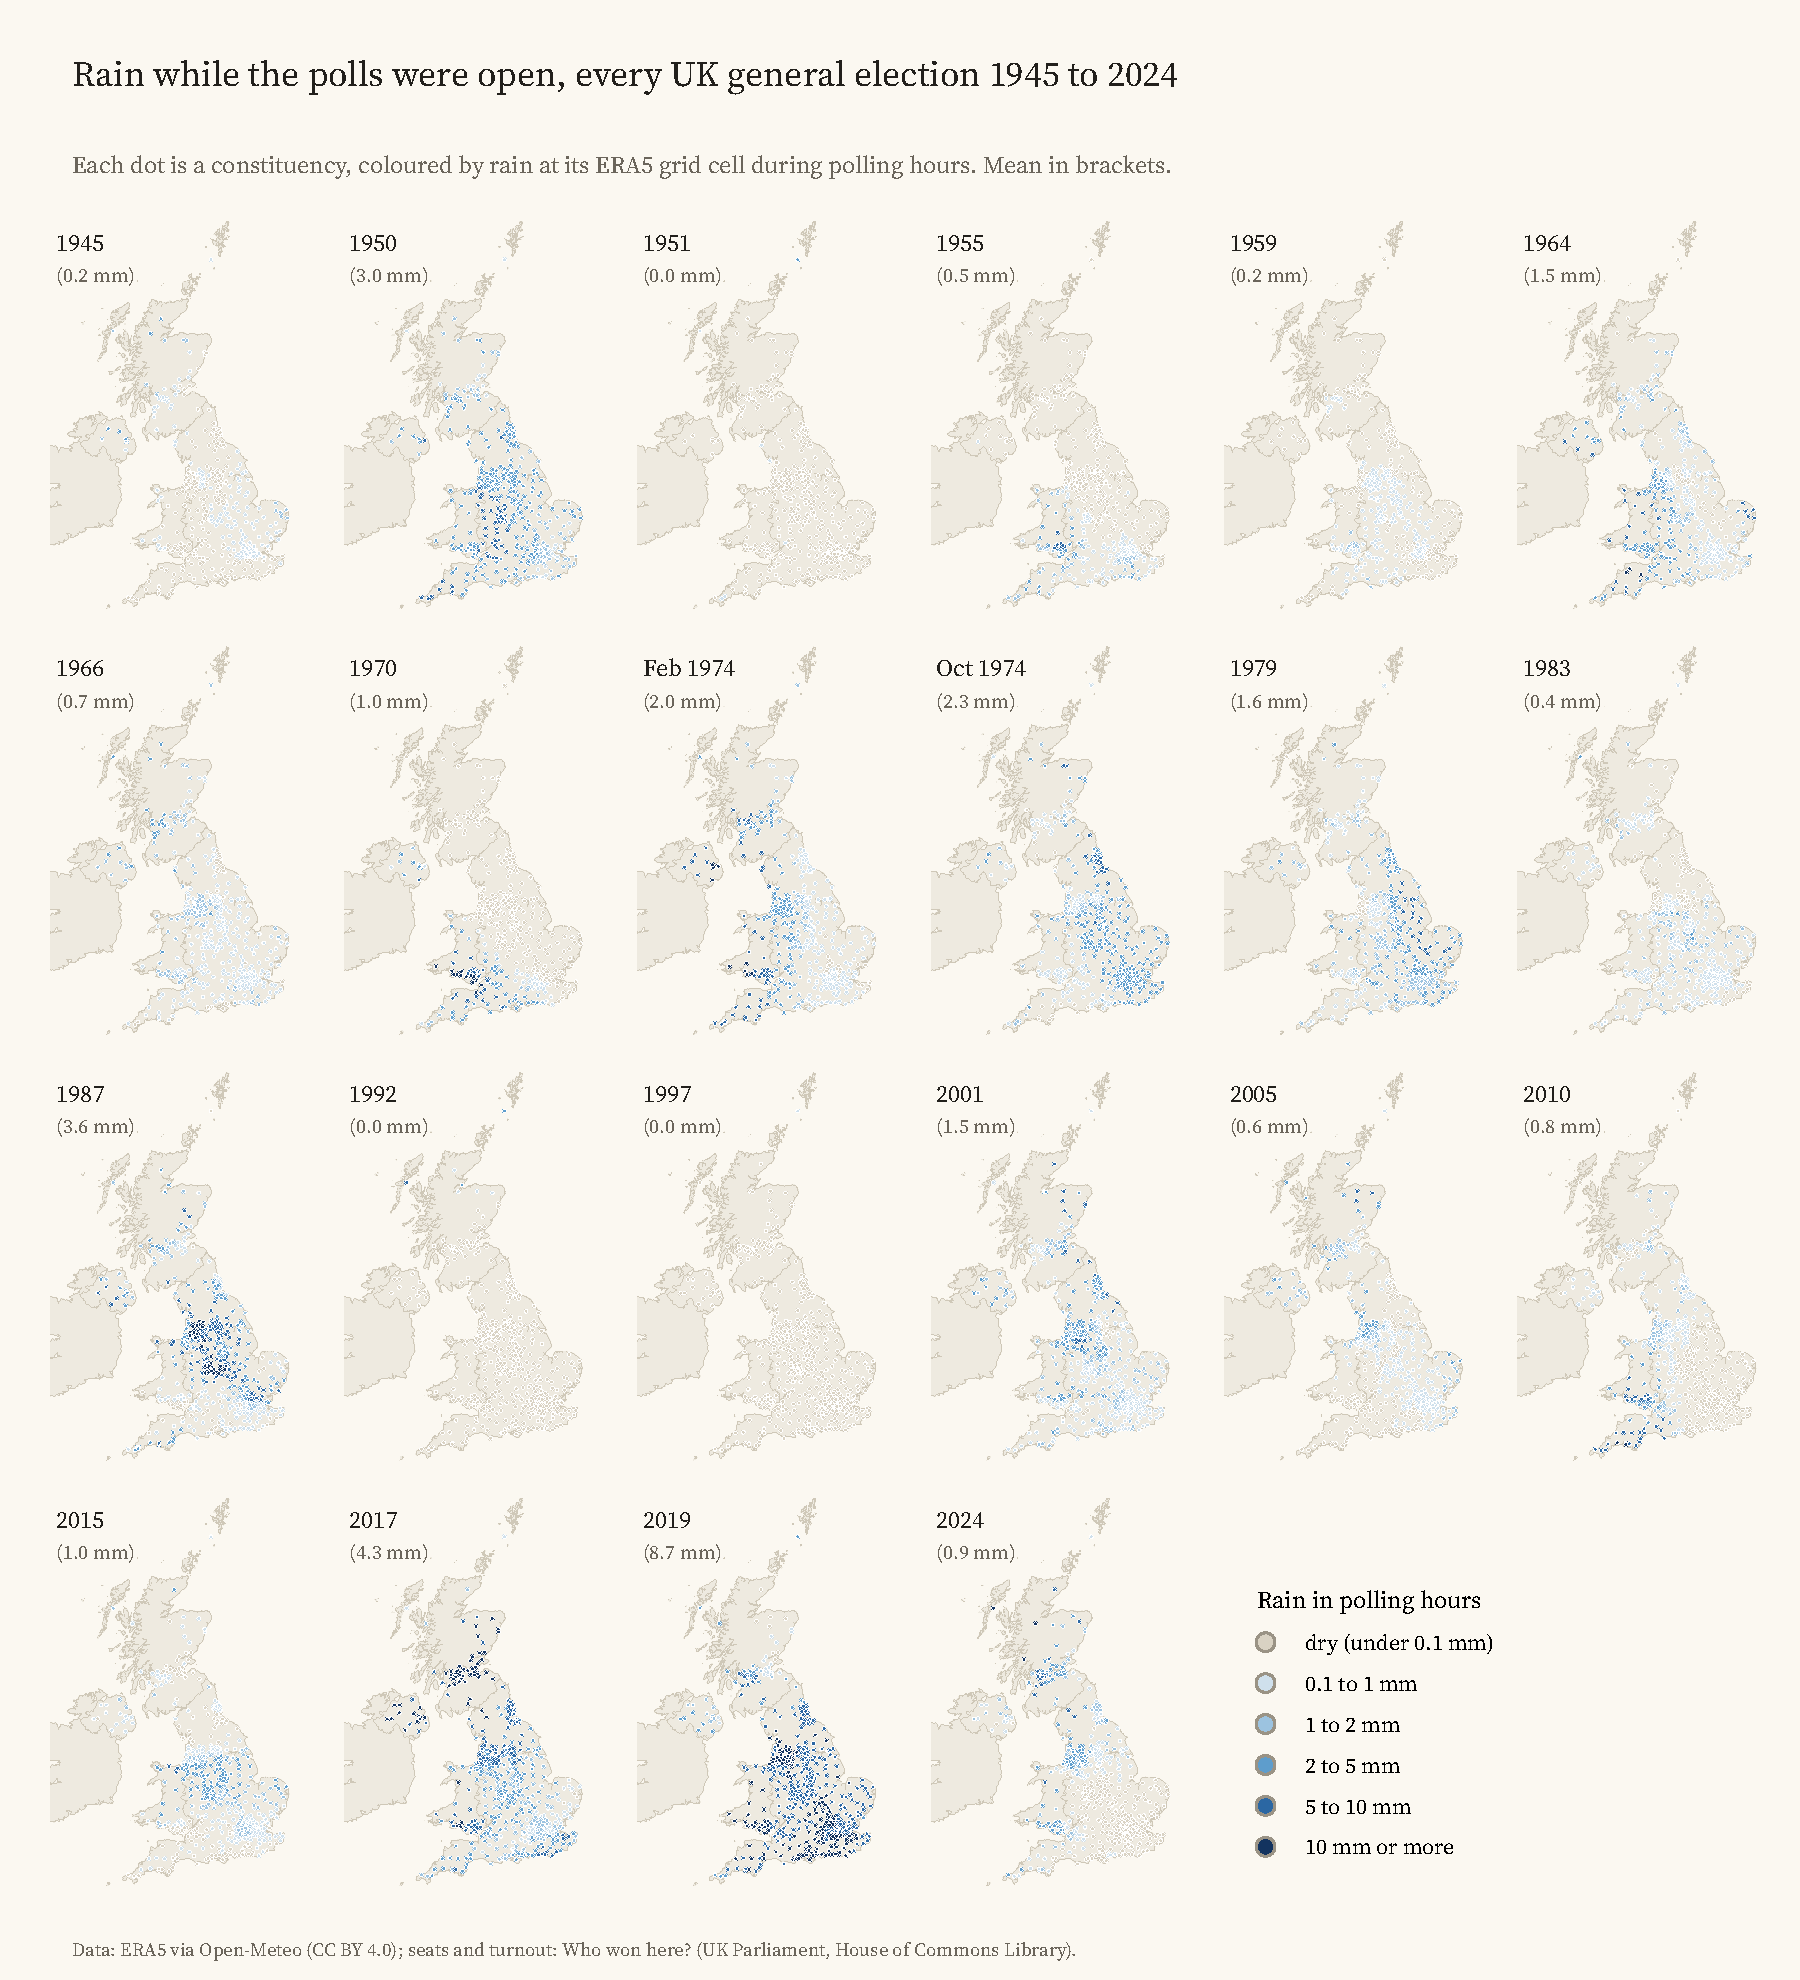
\includegraphics[width=\textwidth]{f_maps.pdf}
\caption{Rain in polling hours at the grid cell of each constituency, every UK general election 1945 to 2024. Mean across seats in brackets.}\label{fig:maps}\end{figure}

\begin{figure}[tbp]\centering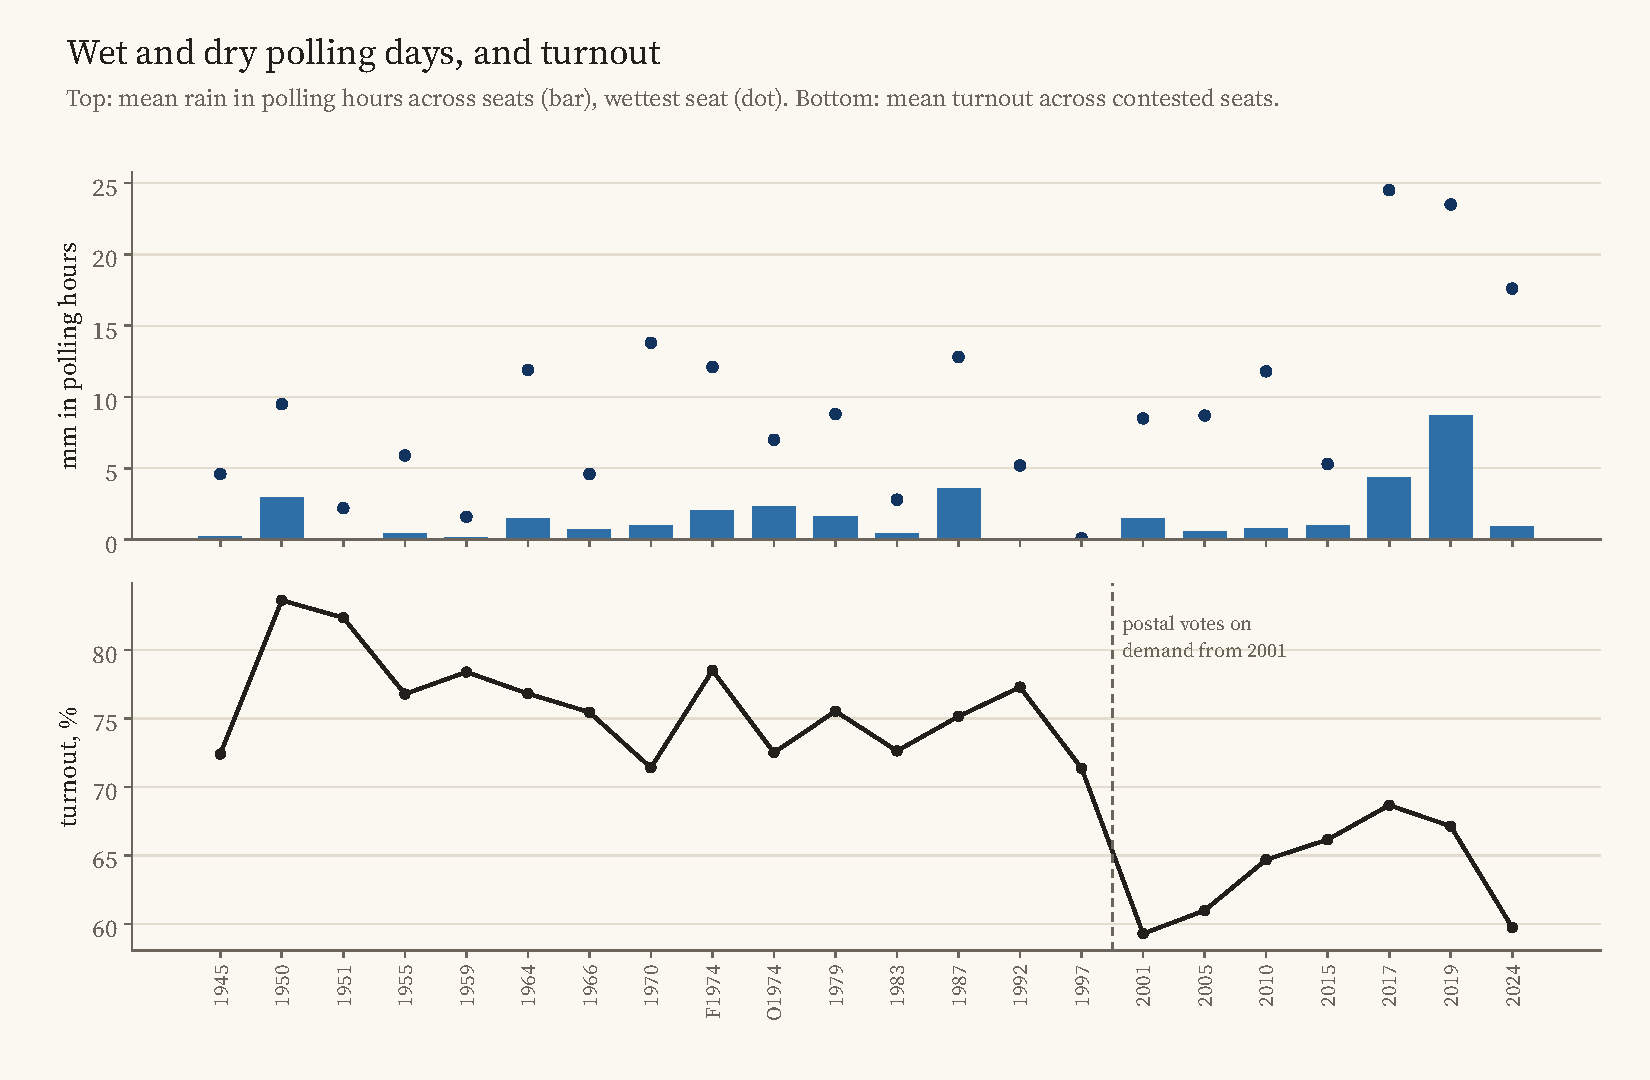
\includegraphics[width=0.95\textwidth]{f_time.pdf}
\caption{Mean polling-hours rain across seats (bars) and in the wettest seat (dots), and mean turnout in contested seats, by election.}\label{fig:time}\end{figure}

\subsection{Main estimate}
Table~\ref{tab:main} reports the main estimate. Each centimetre of polling-hours rain is associated with turnout 0.96 percentage points lower (95\% CI -1.82 to -0.11, $N=13{,}731$). Per millimetre this is -0.096 points; a within-election standard deviation of rain (1.9 mm) corresponds to -0.19 points, and a wet polling day of 5 mm to -0.48 points. Figure~\ref{fig:bins} shows the relationship in binned form, after removing seat and election means. The estimate is close to the Danish estimate of 0.95 points per centimetre \citep{damsbo2023} and larger, per centimetre, than the US estimate of just under one point per inch \citep{gomez2007} or the Dutch estimate of about one point per 25 mm \citep{eisinga2012turnout}.

\begin{table}[tbp]\centering\small\caption{Main estimate (H1) and inference allowing for few elections.}\label{tab:main}
\begin{tabular}{p{7.6cm}rcrr}\toprule Specification & Estimate & 95\% CI & $p$ & $N$\\\midrule
Main: seat and election FE, two-way clustered & -0.96 & [-1.82, -0.11] & 0.028 & 13,731\\
Same, clustered by election $\times$ region only & -0.96 & [-1.86, -0.07] & 0.035 & 13,731\\
Same, clustered by election only (22 clusters) & -0.96 & [-2.17, 0.25] & 0.113 & 13,731\\
Wild cluster bootstrap by election (Webb weights, 9,999 draws) & & & 0.143 & \\
Randomisation inference: rain maps permuted between elections (1,000) & & [-1.12, 1.18] & 0.099 & \\
\bottomrule\end{tabular}\par\vspace{2pt}\parbox{\linewidth}{\footnotesize Turnout in percentage points per centimetre of polling-hours rain. Seat and election fixed effects; standard errors clustered two ways, by seat lineage and by election $\times$ region, unless stated. For randomisation inference the bracket is the central 95\% of the permutation distribution under the sharp null.}\end{table}

\begin{figure}[tbp]\centering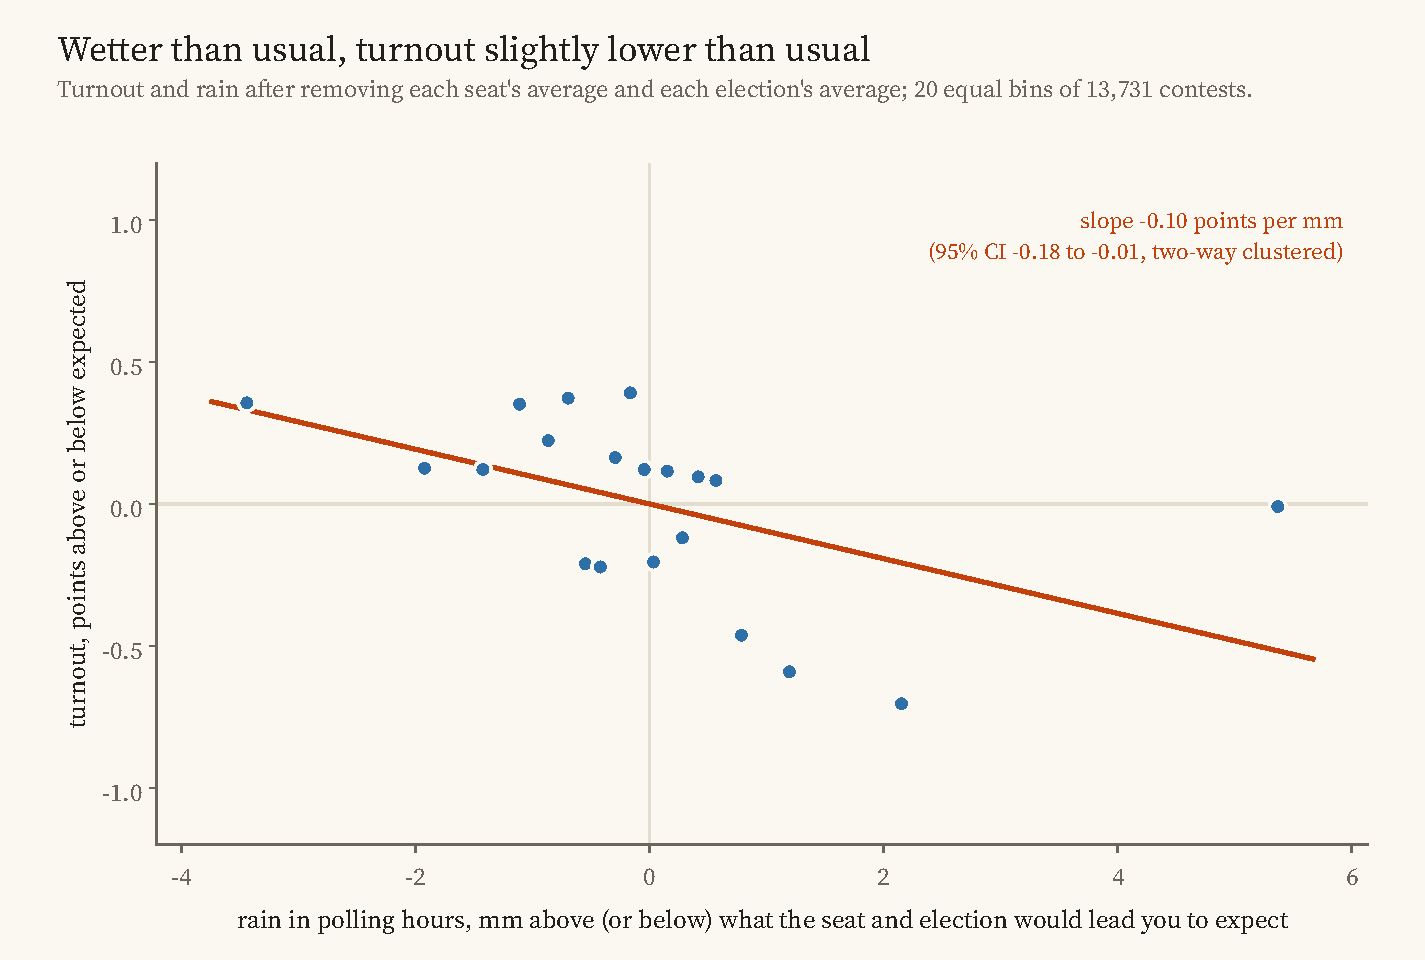
\includegraphics[width=0.85\textwidth]{f_bins.pdf}
\caption{Binned scatter of turnout against polling-hours rain, both net of seat and election fixed effects (20 equal-count bins). The line has the slope of the main estimate.}\label{fig:bins}\end{figure}

\subsection{How much do 22 elections allow us to say?}
The lower panel of Table~\ref{tab:main} reports inference that allows for the small number of elections. Clustering by election alone widens the interval to -2.17 to 0.25. The wild cluster bootstrap by election gives $p=0.14$. Randomisation inference, which swaps the rain maps of real polling days between elections, gives $p=0.10$: 9.9\% of the 1{,}000 permuted estimates were at least as far from zero as the real one, and the middle 95\% of the permutation distribution runs from -1.12 to 1.18 (Figure~\ref{fig:ri}). By these standards the effect is not established. The width of the permutation distribution is itself informative: weather maps that have nothing to do with the election in question produce estimates as large as one point per centimetre with some regularity, because rain on any given day is concentrated in a few regions whose turnout may differ from expectation for other reasons.

\begin{figure}[tbp]\centering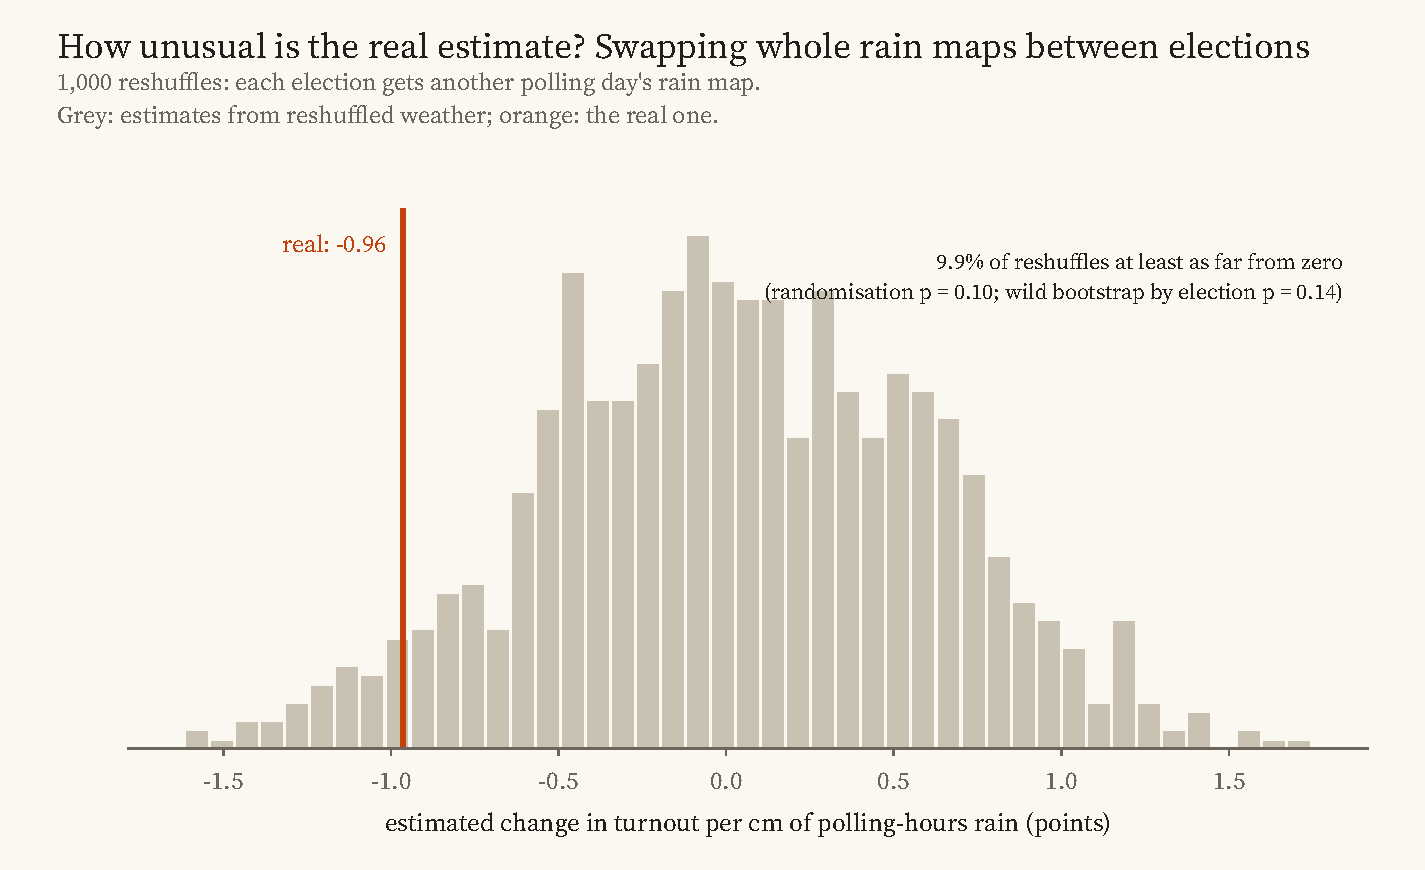
\includegraphics[width=0.85\textwidth]{f_ri.pdf}
\caption{Randomisation inference: estimates from 1{,}000 permutations of whole national rain maps between elections (grey) and the real estimate (orange).}\label{fig:ri}\end{figure}

\subsection{Party shares}
H3 is not supported. In Great Britain, polling-hours rain has no detectable association with the Conservative share (-0.24 points per centimetre, 95\% CI -1.70 to 1.22) or the Labour share (-0.27, CI -4.11 to 3.57); the Conservative minus Labour gap moves by 0.01 points (CI -4.06 to 4.07). With election $\times$ region fixed effects, the intervals narrow but still include zero (Table~\ref{tab:het}). If rain lowers turnout by around a point per centimetre, a partisan effect would have to be implausibly lopsided to be detectable in shares, so this null is expected; but it gives no support to the idea that rain helps the right in Britain.

\subsection{Heterogeneity}
Figure~\ref{fig:het} and Table~\ref{tab:het} report the planned heterogeneity analyses. H2 is contradicted in sign: the association is -0.49 (CI -1.47 to 0.48) for 1945 to 1997 and -1.10 (CI -2.02 to -0.18) for 2001 to 2024, and the interaction in a pooled model is -1.84 (CI -3.46 to -0.21; Holm-adjusted $p=0.11$). The later period contains the two wettest elections and much more within-election variation in rain, so this difference should not be over-read. By nation, the estimate is negative in England, Scotland and Wales and imprecise in Northern Ireland. Crowded and less crowded seats, and marginal and safer seats, show similar estimates, and neither interaction is distinguishable from zero. Temperature, entered with rain, is associated with lower turnout on warmer days (-1.87 points per 10$^\circ$C, CI -3.65 to -0.09; Holm-adjusted $p=0.12$), the opposite of the Dutch and Canadian findings; I treat this as unresolved.

\begin{figure}[tbp]\centering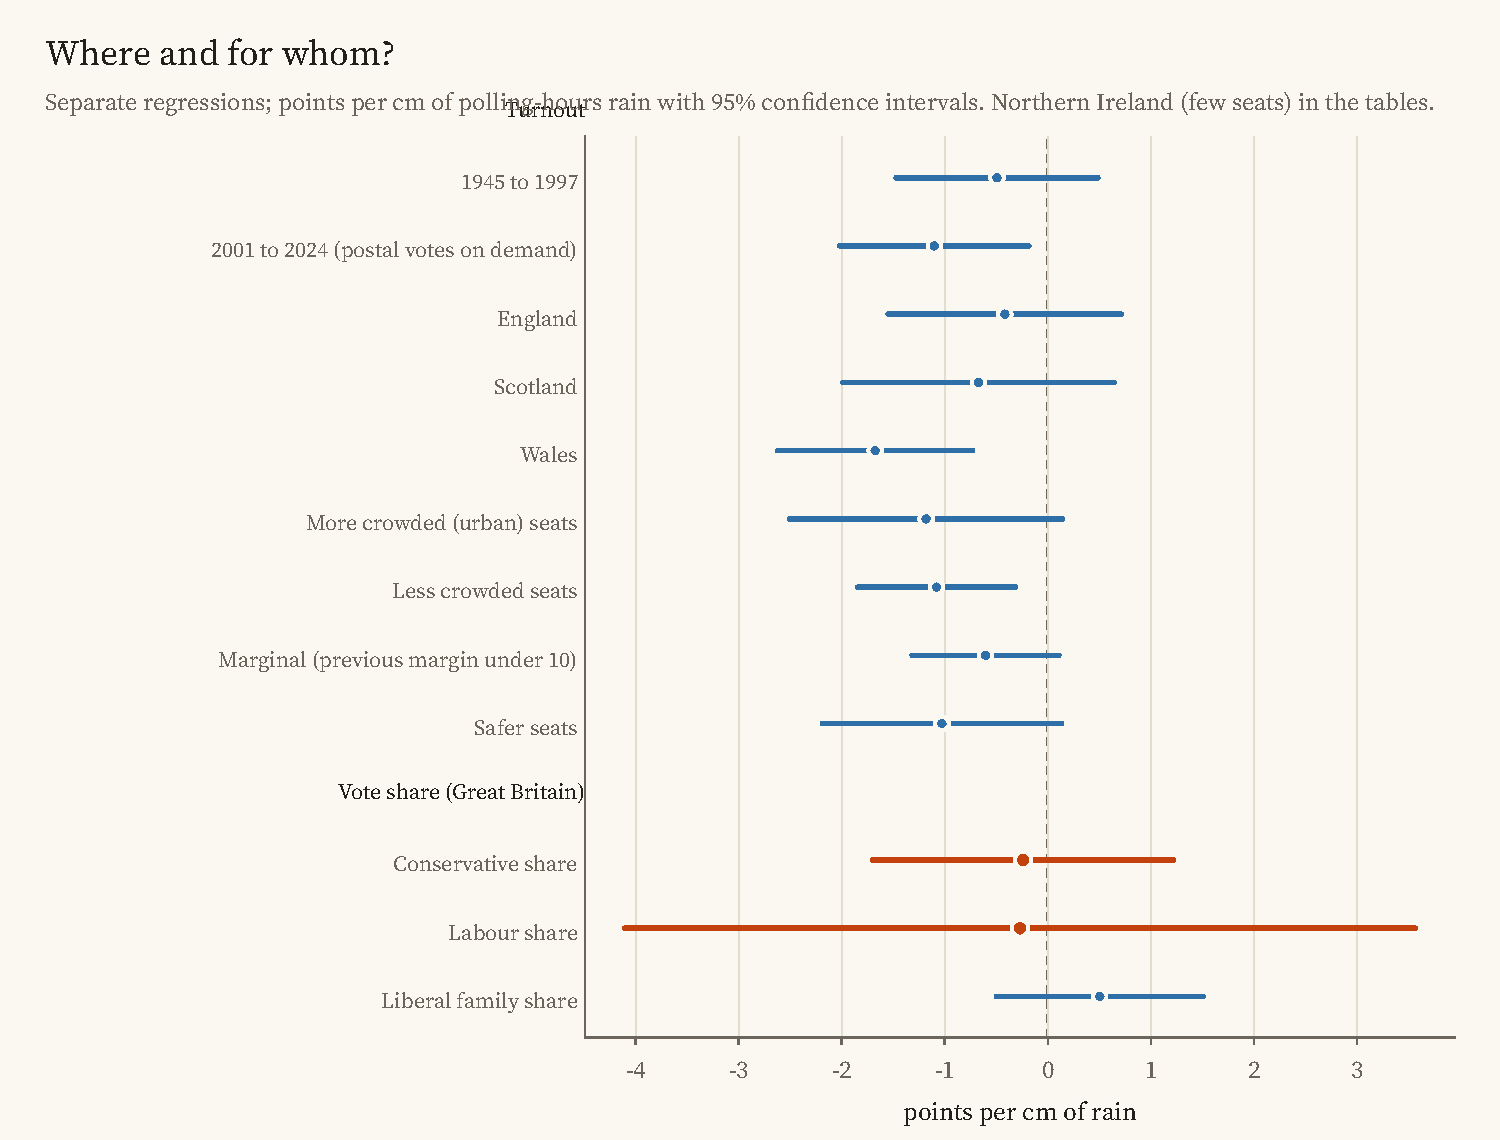
\includegraphics[width=0.85\textwidth]{f_het.pdf}
\caption{Heterogeneity and party shares: separate regressions, points per centimetre of polling-hours rain with 95\% confidence intervals.}\label{fig:het}\end{figure}

\begin{table}[tbp]\centering\small\caption{Heterogeneity (H2, H4) and party shares (H3).}\label{tab:het}
\begin{tabular}{p{7.6cm}rcrr}\toprule Specification & Estimate & 95\% CI & $p$ & $N$\\\midrule
1945 to 1997 & -0.49 & [-1.47, 0.48] & 0.321 & 9,231\\
2001 to 2024 & -1.10 & [-2.02, -0.18] & 0.019 & 4,296\\
Rain x 2001 on (postal votes on demand) & -1.84 & [-3.46, -0.21] & 0.027 & 13,731\\
England & -0.42 & [-1.55, 0.71] & 0.468 & 11,180\\
Scotland & -0.67 & [-1.99, 0.64] & 0.300 & 1,440\\
Wales & -1.68 & [-2.62, -0.73] & 0.001 & 798\\
Northern Ireland & 0.58 & [-3.39, 4.55] & 0.763 & 313\\
Urban (crowded) seats & -1.18 & [-2.51, 0.14] & 0.080 & 6,497\\
Less crowded seats & -1.08 & [-1.84, -0.32] & 0.006 & 7,212\\
Rain x urban (crowded) seat & 0.36 & [-0.76, 1.49] & 0.525 & 13,731\\
Marginal seats & -0.60 & [-1.32, 0.11] & 0.095 & 3,119\\
Safer seats & -1.03 & [-2.19, 0.13] & 0.082 & 9,000\\
Rain x marginal (previous margin under 10 points) & -0.13 & [-0.89, 0.62] & 0.727 & 12,349\\
Temperature, per 10 degrees C (with rain) & -1.87 & [-3.65, -0.09] & 0.040 & 13,731\\
\midrule
Conservative share & -0.24 & [-1.70, 1.22] & 0.747 & 13,113\\
Conservative share, election x region FE & -0.74 & [-1.80, 0.31] & 0.165 & 13,113\\
Conservative share, 1945 to 1997 & -0.61 & [-2.53, 1.30] & 0.529 & 8,748\\
Labour share & -0.27 & [-4.11, 3.57] & 0.890 & 13,387\\
Labour share, election x region FE & -0.76 & [-1.95, 0.43] & 0.212 & 13,387\\
Labour share, 1945 to 1997 & -0.01 & [-2.19, 2.18] & 0.996 & 9,021\\
Liberal family share & 0.50 & [-0.50, 1.50] & 0.322 & 10,571\\
Liberal family share, election x region FE & 0.81 & [-0.26, 1.87] & 0.136 & 10,570\\
Conservative minus Labour share & 0.01 & [-4.06, 4.07] & 0.998 & 13,096\\
\bottomrule\end{tabular}\par\vspace{2pt}\parbox{\linewidth}{\footnotesize Turnout in percentage points per centimetre of polling-hours rain. Seat and election fixed effects; standard errors clustered two ways, by seat lineage and by election $\times$ region, unless stated. Interaction rows report the interaction term. Party shares: percentage points of the vote, single-member contests in Great Britain where the party stood. Holm-adjusted $p$ for H2 to H4: rain x 2001 on 0.11, temperature 0.12, Conservative share 1.00, Labour share 1.00.}\end{table}

\section{Robustness}\label{sec:rob}
\subsection{Specification and measurement}
Figure~\ref{fig:robust} and Table~\ref{tab:rob} report the planned checks. The estimate is negative in every alternative: between -1.12 and -0.55 with other fixed effects or first differences (3 of 6 intervals exclude zero), and between -1.11 and -0.93 for the alternative continuous measures of rain. The first-difference design in seats with unchanged boundaries gives -1.09 (CI -2.10 to -0.07, $N=8{,}903$). With election $\times$ region fixed effects, which compare only seats in the same region at the same election, the estimate is -0.71 (CI -1.28 to -0.14); with election $\times$ nation fixed effects it is -0.55 and the interval includes zero. Whole-day rain gives -1.08 and the 50 km smoothed field -1.11, so the result does not depend on the exact hours or on grid-scale noise. The threshold indicators tell a less tidy story: at least 1 mm is associated with -0.53 points (CI -0.95 to -0.12), but at least 5 mm (-0.33) and at least 10 mm (-0.22) are smaller and imprecise. There is no sign that heavy rain matters more than light rain, which sits uneasily with a simple cost mechanism.

\begin{figure}[tbp]\centering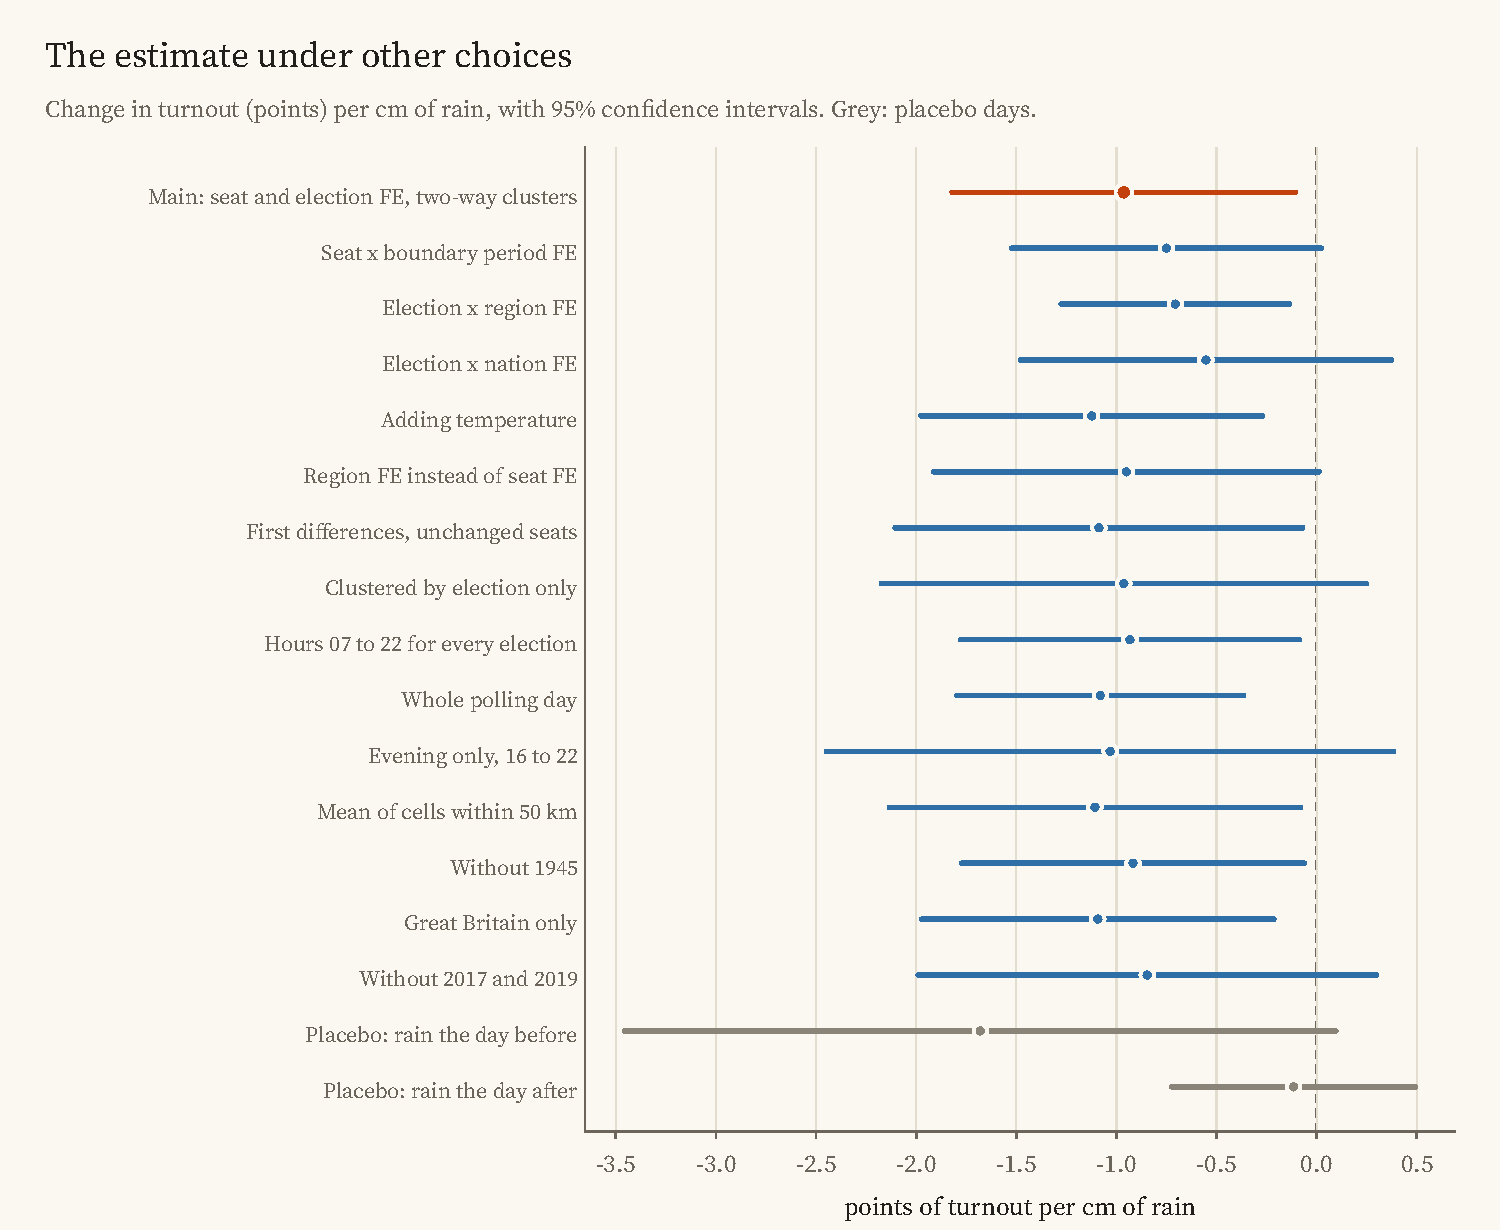
\includegraphics[width=0.85\textwidth]{f_robust.pdf}
\caption{The estimate under alternative specifications and measures, with placebo days (grey). Points per centimetre of rain, 95\% confidence intervals.}\label{fig:robust}\end{figure}

\begin{table}[tbp]\centering\small\caption{Robustness: specifications, measures of rain, samples and placebo days.}\label{tab:rob}
\begin{tabular}{p{7.6cm}rcrr}\toprule Specification & Estimate & 95\% CI & $p$ & $N$\\\midrule
Seat x boundary period FE & -0.75 & [-1.52, 0.02] & 0.057 & 12,749\\
Election x region FE & -0.71 & [-1.28, -0.14] & 0.015 & 13,731\\
Election x nation FE & -0.55 & [-1.48, 0.37] & 0.241 & 13,731\\
Adding temperature and its square & -1.12 & [-1.98, -0.27] & 0.010 & 13,731\\
Region FE instead of seat FE & -0.95 & [-1.91, 0.01] & 0.053 & 14,052\\
First differences, unchanged seats & -1.09 & [-2.10, -0.07] & 0.036 & 8,903\\
\midrule
07 to 22 hours for every election & -0.93 & [-1.78, -0.09] & 0.031 & 13,731\\
Whole polling day (00 to 24) & -1.08 & [-1.80, -0.37] & 0.003 & 13,731\\
Evening only (16 to 22) & -1.03 & [-2.45, 0.38] & 0.153 & 13,731\\
Mean of cells within 50 km & -1.11 & [-2.13, -0.08] & 0.035 & 13,731\\
log(1 + mm) (per unit) & -0.50 & [-0.85, -0.15] & 0.005 & 13,731\\
At least 1 mm (indicator) (points) & -0.53 & [-0.95, -0.12] & 0.011 & 13,731\\
At least 5 mm (indicator) (points) & -0.33 & [-0.94, 0.28] & 0.292 & 13,731\\
At least 10 mm (indicator) (points) & -0.22 & [-1.26, 0.82] & 0.681 & 13,731\\
\midrule
Without 1945 & -0.92 & [-1.77, -0.06] & 0.036 & 13,274\\
Great Britain only & -1.09 & [-1.97, -0.21] & 0.015 & 13,418\\
Without 2017 and 2019 & -0.85 & [-1.99, 0.30] & 0.146 & 12,431\\
\midrule
Placebo: day before, alone & -1.68 & [-3.46, 0.10] & 0.064 & 13,731\\
Placebo: day after, alone & -0.12 & [-0.72, 0.49] & 0.709 & 13,731\\
Joint: polling day & -0.86 & [-1.73, 0.01] & 0.051 & 13,731\\
Joint: day before & -1.58 & [-3.40, 0.24] & 0.088 & 13,731\\
Joint: day after & 0.04 & [-0.53, 0.62] & 0.877 & 13,731\\
\bottomrule\end{tabular}\par\vspace{2pt}\parbox{\linewidth}{\footnotesize Turnout in percentage points per centimetre of polling-hours rain. Seat and election fixed effects; standard errors clustered two ways, by seat lineage and by election $\times$ region, unless stated. Indicator rows give points for a contest with at least that much rain. The first-difference row relates the change in turnout to the change in rain between consecutive elections in seats with unchanged boundaries, with election FE.}\end{table}

\subsection{Placebos}
Rain on the day before polling day, over the same hours, is associated with turnout -1.68 points per centimetre (CI -3.46 to 0.10); rain on the day after with -0.12 (CI -0.72 to 0.49). Entered together, polling-day rain is -0.86 (CI -1.73 to 0.01) and the day before -1.58 (CI -3.40 to 0.24). Within elections, rain on polling day is only weakly correlated with rain the day before ($r=0.14$) and the day after ($r=0.08$), so the day-before association is not simply the polling-day effect showing through. The after-day placebo behaves as it should; the before-day placebo does not. There are two readings. Wet weather on the eve of polling may genuinely reduce turnout, by hampering the final day of canvassing and knocking-up, by deterring postal voters from posting their ballots, or through mood. Or the pattern of rain across seats around polling day may be correlated with unobserved local influences on turnout in that year. The design cannot distinguish these, and the second reading counsels against interpreting $\beta$ as a clean causal effect.

\subsection{Leave one out}
Dropping any single election leaves the estimate between -1.49 and -0.75, and dropping any single region between -1.13 and -0.57 (Figure~\ref{fig:loo}; Table~\ref{tab:loo} in the appendix); 18 of 22 and 10 of 12 intervals exclude zero. Without 2017 and 2019 the estimate is -0.85 (CI -1.99 to 0.30). Without Scotland it falls to -0.57. No single election or region drives the sign, but the precision depends on the wet elections.

\begin{figure}[tbp]\centering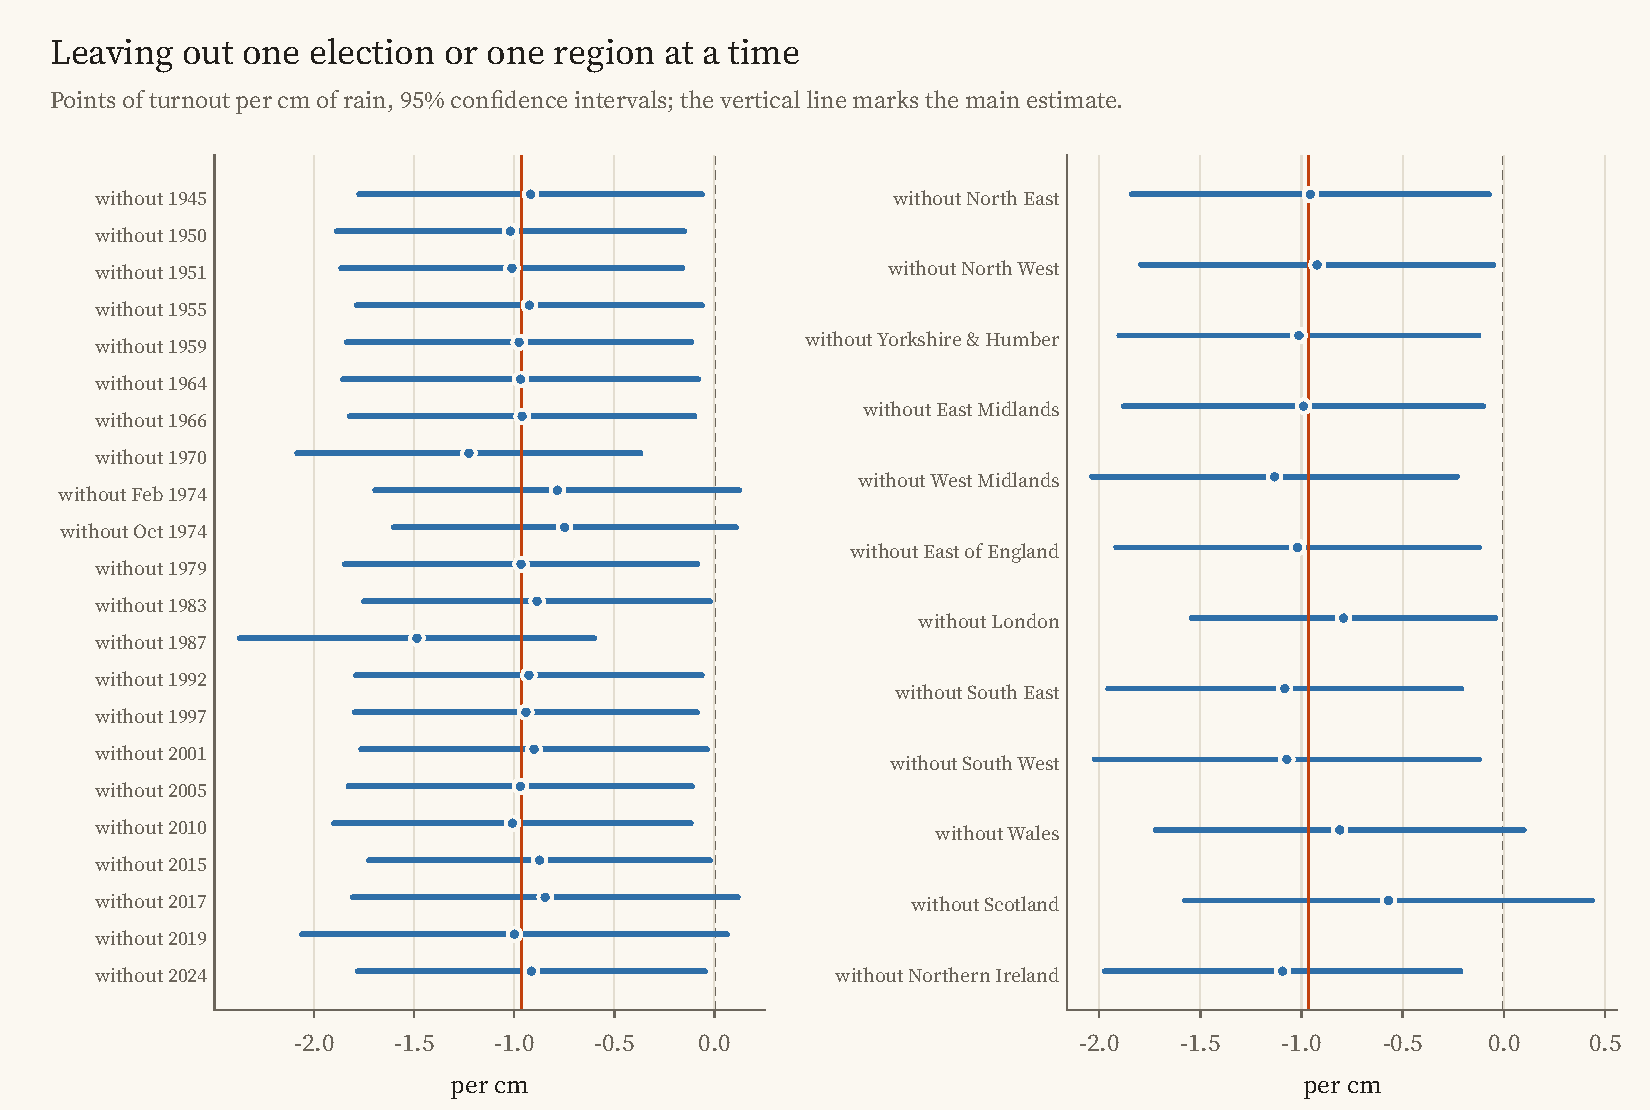
\includegraphics[width=\textwidth]{f_loo.pdf}
\caption{Leave one election out (left) and leave one region out (right). Points per centimetre of rain, 95\% confidence intervals; the vertical line marks the main estimate.}\label{fig:loo}\end{figure}

\subsection{Exploratory checks}\label{sec:explore}
The following checks were not in the plan; they were added at an independent review and are exploratory. First, the day-before placebo was put through the same few-cluster inference as the main estimate: the wild cluster bootstrap by election gives $p=0.08$ and randomisation inference with the same map swaps applied to the day before gives $p=0.04$, both smaller than for polling-day rain ($p=0.14$ and 0.10). By these standards the placebo is at least as unusual as the main estimate, which weighs against reading $\beta$ as the effect of rain on the cost of getting to the polls. Second, with election $\times$ region fixed effects the wild cluster bootstrap by election gives $p=0.05$ for an estimate of -0.71. Third, because many seats share a grid cell and therefore share their rain, I collapsed the data to one row per cell and election (mean turnout of the seats in the cell; 6{,}194 rows, 367 cells) with cell and election fixed effects: the estimate is -1.17 (CI -1.93 to -0.41, clustered by cell and by election $\times$ region). This confirms that the result is not an artefact of counting a shared cell many times, but it does not address the small number of elections.

\section{Discussion}\label{sec:disc}
Three conclusions follow. First, the effect of rain on turnout in British general elections is at most small. Even the lower end of the conventional interval, -1.82 points per centimetre, implies that a 5 mm polling day costs less than one point of turnout; and the national averages in Figure~\ref{fig:time} show that weather is a minor influence on turnout compared with the changes in competition and partisanship that dominate British turnout history \citep{heath2007,franklin2004}. If the main estimate were correct and applied uniformly, the rain of December 2019, the wettest polling day in the series, would correspond to about 0.84 points of national turnout. That is not nothing in a close election, but it is far from the scale implied by election-night commentary.

Second, whether there is a small effect at all is uncertain. The conventional estimate excludes zero, but inference that respects the 22 elections does not, and the day-before placebo is as large as the main effect and, by the same few-cluster standards, at least as unusual (Section~\ref{sec:explore}). This is the pattern \citet{cooperman2017} warned of: with spatially correlated weather and few independent draws, conventional standard errors overstate precision. It also echoes the mixed international record, in which careful studies of single countries have found effects \citep{damsbo2023,eisinga2012turnout}, no effects \citep{persson2014} and even positive effects \citep{lind2020}.

Third, the patterns that would make a cost-of-voting story compelling are absent. Heavy rain is not associated with larger falls than light rain, the association does not weaken after postal voting on demand, and there is no partisan effect. Each of these could reflect a lack of power, but together they suggest that whatever links weather and turnout in British seats is not simply the inconvenience of the walk to the polling station.

\subsection{Limitations}
The design has several limits. \emph{Measurement.} ERA5 precipitation has an effective resolution of about 31 km, so dozens of urban seats share one value and convective showers are smoothed away. Classical measurement error in rain attenuates $\beta$ towards zero; the smoothed 50 km exposure gives a similar estimate, which suggests that grid-scale noise is not the main issue, but the reliability of the measure cannot be estimated from these data, and the true seat-level effect may be larger than estimated. \emph{Unit.} Turnout is measured per constituency, so the analysis cannot say who stayed at home; individual-level validated turnout, as in \citet{damsbo2023}, is not available for Britain across this period. \emph{Postal votes.} Postal ballots cast before polling day are included in turnout but were never exposed to polling-day rain; their share has grown since 2001, which should dilute the effect in later elections. \emph{Geography.} Seats are points, boundaries changed, and the seat-name lineage is an approximation to a fixed place. \emph{1945.} The list of postponed seats may be incomplete; dropping 1945 entirely changes the estimate little (-0.92). \emph{Polling hours.} The 1945 hours are uncertain; using 7am to 10pm throughout gives -0.93. \emph{Power.} With a two-way clustered standard error of 0.44, the smallest effect detectable with 80\% power at the 5\% level is about 1.2 points per centimetre; under clustering by election it is about 1.6. Effects of the size found elsewhere are therefore near the limit of what 22 British elections can detect. \emph{Exclusion.} As \citet{mellon2025} documents, weather affects many things; the estimates are reduced-form associations of weather with turnout and should not be used as an instrument for turnout.

\section{Conclusion}\label{sec:concl}
Does rain keep Britain at home? Across 22 general elections and 14{,}052 constituency contests, seats that were wetter than usual during polling hours had slightly lower turnout than usual, by about a tenth of a point per millimetre. The association is consistent in sign but not robust to inference that respects the small number of elections, a placebo day shows an association as large, and there is no partisan effect. The safest reading is that rain has at most a small effect on British turnout, and that claims of elections decided by the weather should be treated with scepticism. Future work could use finer weather data (radar-based rainfall for recent elections), individual-level turnout records, or local elections, which are more numerous and would supply many more independent weather draws.

\section*{Data availability statement}
Data and code: Zenodo DOI https://doi.org/10.5281/zenodo.24094534. The replication files include the seat-election panel with all weather measures, the model estimates and the code, also at \url{https://github.com/Tristan-Hotham/polling-rain}; an interactive map is at \url{https://maps.tristanhotham.com/polling-rain/}. Weather data are from Open-Meteo (CC BY 4.0) based on ERA5 (Copernicus Climate Change Service); election results contain Parliamentary information licensed under the Open Parliament Licence v3.0.

\section*{AI assistance}
I wrote the text, with drafting and editing assistance from Claude (Anthropic), which also helped prepare the analysis code. I reviewed and checked all text and results.

\begin{thebibliography}{99}
\bibitem[Arnold and Freier(2015)]{arnoldfreier2015} Arnold, F. and Freier, R. (2015) The partisan effects of voter turnout: how conservatives profit from rainy election days. DIW Discussion Paper 1463. Berlin: DIW Berlin.
\bibitem[Art\'es(2014)]{artes2014} Art\'es, J. (2014) The rain in Spain: turnout and partisan voting in Spanish elections. \textit{European Journal of Political Economy} 34: 126-141. doi:10.1016/j.ejpoleco.2014.01.005
\bibitem[Bassi(2019)]{bassi2019} Bassi, A. (2019) Weather, risk, and voting: an experimental analysis of the effect of weather on vote choice. \textit{Journal of Experimental Political Science} 6(1): 17-32.
\bibitem[Blais(2006)]{blais2006} Blais, A. (2006) What affects voter turnout? \textit{Annual Review of Political Science} 9: 111-125. doi:10.1146/annurev.polisci.9.070204.105121
\bibitem[Cameron et~al.(2008)]{cameron2008} Cameron, A. C., Gelbach, J. B. and Miller, D. L. (2008) Bootstrap-based improvements for inference with clustered errors. \textit{Review of Economics and Statistics} 90(3): 414-427. doi:10.1162/rest.90.3.414
\bibitem[Cameron et~al.(2011)]{cameron2011} Cameron, A. C., Gelbach, J. B. and Miller, D. L. (2011) Robust inference with multiway clustering. \textit{Journal of Business and Economic Statistics} 29(2): 238-249. doi:10.1198/jbes.2010.07136
\bibitem[Cooperman(2017)]{cooperman2017} Cooperman, A. D. (2017) Randomization inference with rainfall data: using historical weather patterns for variance estimation. \textit{Political Analysis} 25(3): 277-288.
\bibitem[Damsbo-Svendsen and Hansen(2023)]{damsbo2023} Damsbo-Svendsen, S. and Hansen, K. M. (2023) When the election rains out and how bad weather excludes marginal voters from turning out. \textit{Electoral Studies} 81: 102573. doi:10.1016/j.electstud.2022.102573
\bibitem[Denver and Hands(1974)]{denverhands1974} Denver, D. T. and Hands, H. T. G. (1974) Marginality and turnout in British general elections. \textit{British Journal of Political Science} 4(1): 17-35.
\bibitem[Denver and Hands(1985)]{denverhands1985} Denver, D. and Hands, G. (1985) Marginality and turnout in general elections in the 1970s. \textit{British Journal of Political Science} 15(3): 381-388.
\bibitem[Downs(1957)]{downs1957} Downs, A. (1957) \textit{An Economic Theory of Democracy}. New York: Harper and Brothers.
\bibitem[Eisinga et~al.(2012a)]{eisinga2012turnout} Eisinga, R., Te Grotenhuis, M. and Pelzer, B. (2012a) Weather conditions and voter turnout in Dutch national parliament elections, 1971-2010. \textit{International Journal of Biometeorology} 56(4): 783-786. doi:10.1007/s00484-011-0477-7
\bibitem[Eisinga et~al.(2012b)]{eisinga2012party} Eisinga, R., Te Grotenhuis, M. and Pelzer, B. (2012b) Weather conditions and political party vote share in Dutch national parliament elections, 1971-2010. \textit{International Journal of Biometeorology} 56(6): 1161-1165. doi:10.1007/s00484-011-0504-8
\bibitem[Fraga and Hersh(2010)]{fragahersh2010} Fraga, B. and Hersh, E. (2010) Voting costs and voter turnout in competitive elections. \textit{Quarterly Journal of Political Science} 5(4): 339-356. doi:10.1561/100.00010093
\bibitem[Franklin(2004)]{franklin2004} Franklin, M. N. (2004) \textit{Voter Turnout and the Dynamics of Electoral Competition in Established Democracies since 1945}. Cambridge: Cambridge University Press.
\bibitem[Fujiwara et~al.(2016)]{fujiwara2016} Fujiwara, T., Meng, K. and Vogl, T. (2016) Habit formation in voting: evidence from rainy elections. \textit{American Economic Journal: Applied Economics} 8(4): 160-188. doi:10.1257/app.20140533
\bibitem[Funk(2010)]{funk2010} Funk, P. (2010) Social incentives and voter turnout: evidence from the Swiss mail ballot system. \textit{Journal of the European Economic Association} 8(5): 1077-1103.
\bibitem[Garcia Rodriguez and Redmond(2020)]{garciaredmond2020} Garcia Rodriguez, A. and Redmond, P. (2020) Rainfall, population density and voter turnout. \textit{Electoral Studies} 64: 102128. doi:10.1016/j.electstud.2020.102128
\bibitem[Gerber et~al.(2003)]{gerber2003} Gerber, A. S., Green, D. P. and Shachar, R. (2003) Voting may be habit-forming: evidence from a randomized field experiment. \textit{American Journal of Political Science} 47(3): 540-550. doi:10.1111/1540-5907.00038
\bibitem[Geys(2006)]{geys2006} Geys, B. (2006) Explaining voter turnout: a review of aggregate-level research. \textit{Electoral Studies} 25(4): 637-663.
\bibitem[Gomez et~al.(2007)]{gomez2007} Gomez, B. T., Hansford, T. G. and Krause, G. A. (2007) The Republicans should pray for rain: weather, turnout, and voting in U.S. presidential elections. \textit{Journal of Politics} 69(3): 649-663. doi:10.1111/j.1468-2508.2007.00565.x
\bibitem[Hansard(1945a)]{hansard1945a} Hansard (1945a) General Election (Polling Date). HC Deb 31 May 1945, vol. 411, cols 373-374.
\bibitem[Hansard(1945b)]{hansard1945b} Hansard (1945b) Postponement of Polling Day Bill. HC Deb 11 June 1945, vol. 411, cols 1382-1393.
\bibitem[Hansford and Gomez(2010)]{hansfordgomez2010} Hansford, T. G. and Gomez, B. T. (2010) Estimating the electoral effects of voter turnout. \textit{American Political Science Review} 104(2): 268-288.
\bibitem[Heath(2007)]{heath2007} Heath, O. (2007) Explaining turnout decline in Britain, 1964-2005: party identification and the political context. \textit{Political Behavior} 29(4): 493-516. doi:10.1007/s11109-007-9039-4
\bibitem[Hersbach et~al.(2020)]{hersbach2020} Hersbach, H., Bell, B., Berrisford, P. et al. (2020) The ERA5 global reanalysis. \textit{Quarterly Journal of the Royal Meteorological Society} 146(730): 1999-2049. doi:10.1002/qj.3803
\bibitem[Hodler et~al.(2015)]{hodler2015} Hodler, R., Luechinger, S. and Stutzer, A. (2015) The effects of voting costs on the democratic process and public finances. \textit{American Economic Journal: Economic Policy} 7(1): 141-171. doi:10.1257/pol.20120383
\bibitem[Horiuchi and Kang(2018)]{horiuchikang2018} Horiuchi, Y. and Kang, W. C. (2018) Why should the Republicans pray for rain? Electoral consequences of rainfall revisited. \textit{American Politics Research} 46(5): 869-889. doi:10.1177/1532673X17745631
\bibitem[Hotham(2026)]{hotham2026ele} Hotham, T. (2026) Who won here? Every UK general election since 1832 on one map. Zenodo. doi:10.5281/zenodo.23761425
\bibitem[Knack(1994)]{knack1994} Knack, S. (1994) Does rain help the Republicans? Theory and evidence on turnout and the vote. \textit{Public Choice} 79(1-2): 187-209.
\bibitem[Lind(2020)]{lind2020} Lind, J. T. (2020) Rainy day politics: an instrumental variables approach to the effect of parties on political outcomes. \textit{European Journal of Political Economy} 61.
\bibitem[Meier et~al.(2019)]{meier2019} Meier, A. N., Schmid, L. and Stutzer, A. (2019) Rain, emotions and voting for the status quo. \textit{European Economic Review} 119: 434-451. doi:10.1016/j.euroecorev.2019.07.014
\bibitem[Mellon(2025)]{mellon2025} Mellon, J. (2025) Rain, rain, go away: 194 potential exclusion-restriction violations for studies using weather as an instrumental variable. \textit{American Journal of Political Science} 69(3). doi:10.1111/ajps.12894
\bibitem[Mu\~noz-Sabater et~al.(2021)]{munozsabater2021} Mu\~noz-Sabater, J., Dutra, E., Agust\'i-Panareda, A. et al. (2021) ERA5-Land: a state-of-the-art global reanalysis dataset for land applications. \textit{Earth System Science Data} 13: 4349-4383. doi:10.5194/essd-13-4349-2021
\bibitem[Persson et~al.(2014)]{persson2014} Persson, M., Sundell, A. and \"Ohrvall, R. (2014) Does Election Day weather affect voter turnout? Evidence from Swedish elections. \textit{Electoral Studies} 33: 335-342. doi:10.1016/j.electstud.2013.07.021
\bibitem[Rallings and Thrasher(2007)]{ralling2007} Rallings, C. and Thrasher, M. (2007) \textit{British Electoral Facts 1832-2006}. Aldershot: Ashgate.
\bibitem[Rallings et~al.(2010)]{ralling2010} Rallings, C., Thrasher, M. and Borisyuk, G. (2010) Much ado about not very much: the electoral consequences of postal voting at the 2005 British general election. \textit{British Journal of Politics and International Relations} 12(2): 223-238. doi:10.1111/j.1467-856X.2010.00403.x
\bibitem[Riker and Ordeshook(1968)]{rikerordeshook1968} Riker, W. H. and Ordeshook, P. C. (1968) A theory of the calculus of voting. \textit{American Political Science Review} 62(1): 25-42.
\bibitem[Stockemer and Wigginton(2018)]{stockemerwigginton2018} Stockemer, D. and Wigginton, M. (2018) Fair weather voters: do Canadians stay at home when the weather is bad? \textit{International Journal of Biometeorology} 62(6): 1027-1037. doi:10.1007/s00484-018-1506-6
\bibitem[Webb(2023)]{webb2023} Webb, M. D. (2023) Reworking wild bootstrap-based inference for clustered errors. \textit{Canadian Journal of Economics} 56(3): 839-858.
\bibitem[White(2012)]{white2012} White, I. (2012) \textit{Polling Stations and Hours of Polling}. House of Commons Library Standard Note SN/PC/05517. London: House of Commons Library.
\bibitem[Zippenfenig(2023)]{zippenfenig2023} Zippenfenig, P. (2023) Open-Meteo.com Weather API [computer software]. Zenodo. doi:10.5281/zenodo.7970649
\end{thebibliography}

\appendix
\section{Full tables and data construction}
\subsection{Data construction}
Contests are those of \citet{hotham2026ele} for the 22 general elections from 1945 to 2024 (14,090 rows). Seat points (longitude, latitude) were rounded to the nearest 0.25 degree to give 369 cells; every contest matched a weather record. For each cell and polling date the Open-Meteo archive returned 72 hourly values of precipitation (mm, total of the preceding hour) and 2 m temperature from 00:00 local time (Europe/London) on the day before. With $s$ and $e$ the opening and closing hours, polling-hours rain is the sum of values with indices $25+s$ to $24+e$ (0-based); the day-before and day-after placebos use the same hours shifted by 24 hours, and whole-day rain the hours 00:00 to 24:00. Seat lineage is the constituency name lower-cased with punctuation removed. Region is the ONS region containing the seat point (nearest region for points offshore), or the nation for Scotland, Wales and Northern Ireland. Seat crowding is the number of other constituency points within 15 km at the same election. Previous margin is the winner's share minus the runner-up's share at the previous election under the same name (single-member contests). Party families follow \citet{hotham2026ele}. The 1945 seats dropped as postponed are: Carlisle, Bolton, Farnworth, Nelson and Colne, Darwen, Westhoughton, Barrow in Furness, Lonsdale, Crewe, Edinburgh Central, Edinburgh North, Edinburgh East, Edinburgh South, Edinburgh West, Midlothian and Peebles Northern, Greenock, Stirling and Falkirk, West Renfrewshire, Peebles and South Midlothian, Berwick and Haddington, Clackmannan and East Stirlingshire, Warrington.

\begin{table}[tbp]\centering\small\caption{Weather and turnout by election (analysis sample).}\label{tab:elec}
\begin{tabular}{lcrrrrrrr}\toprule Election & Hours & $N$ & Rain mean & SD & Max & $\geq$5 mm \% & Temp. $^\circ$C & Turnout \%\\\midrule
1945 & 08 to 21 & 588 & 0.20 & 0.42 & 4.6 & 0.0 & 20.4 & 72.4\\
1950 & 07 to 21 & 623 & 2.98 & 1.61 & 9.5 & 12.5 & 5.7 & 83.6\\
1951 & 07 to 21 & 621 & 0.00 & 0.09 & 2.2 & 0.0 & 7.0 & 82.4\\
1955 & 07 to 21 & 630 & 0.45 & 0.97 & 5.9 & 1.4 & 12.5 & 76.8\\
1959 & 07 to 21 & 630 & 0.15 & 0.24 & 1.6 & 0.0 & 15.8 & 78.4\\
1964 & 07 to 21 & 630 & 1.46 & 1.72 & 11.9 & 4.3 & 7.6 & 76.8\\
1966 & 07 to 21 & 630 & 0.70 & 0.65 & 4.6 & 0.0 & 7.9 & 75.5\\
1970 & 07 to 22 & 630 & 0.97 & 2.51 & 13.8 & 7.3 & 18.7 & 71.4\\
February 1974 & 07 to 22 & 635 & 2.02 & 2.48 & 12.1 & 11.7 & 2.2 & 78.5\\
October 1974 & 07 to 22 & 635 & 2.30 & 1.63 & 7.0 & 3.3 & 7.4 & 72.5\\
1979 & 07 to 22 & 635 & 1.60 & 1.38 & 8.8 & 3.3 & 5.2 & 75.5\\
1983 & 07 to 22 & 650 & 0.45 & 0.43 & 2.8 & 0.0 & 14.9 & 72.6\\
1987 & 07 to 22 & 650 & 3.60 & 3.69 & 12.8 & 30.8 & 12.3 & 75.2\\
1992 & 07 to 22 & 651 & 0.02 & 0.29 & 5.2 & 0.2 & 11.5 & 77.3\\
1997 & 07 to 22 & 659 & 0.00 & 0.00 & 0.1 & 0.0 & 16.1 & 71.4\\
2001 & 07 to 22 & 659 & 1.49 & 1.44 & 8.5 & 2.7 & 11.3 & 59.3\\
2005 & 07 to 22 & 646 & 0.59 & 0.95 & 8.7 & 0.5 & 11.7 & 61.0\\
2010 & 07 to 22 & 650 & 0.79 & 1.73 & 11.8 & 4.9 & 9.8 & 64.7\\
2015 & 07 to 22 & 650 & 0.98 & 1.14 & 5.3 & 0.5 & 10.5 & 66.2\\
2017 & 07 to 22 & 650 & 4.35 & 4.26 & 24.5 & 31.7 & 14.7 & 68.7\\
2019 & 07 to 22 & 650 & 8.70 & 3.85 & 23.5 & 88.3 & 5.6 & 67.1\\
2024 & 07 to 22 & 650 & 0.90 & 1.68 & 17.6 & 3.1 & 14.8 & 59.7\\
\bottomrule\end{tabular}\par\vspace{2pt}\parbox{\linewidth}{\footnotesize Rain in mm over polling hours at the seat's grid cell; temperature is the mean over polling hours.}\end{table}

\begin{table}[tbp]\centering\small\caption{Leave one election or one region out.}\label{tab:loo}
\begin{tabular}{p{7.6cm}rcrr}\toprule Specification & Estimate & 95\% CI & $p$ & $N$\\\midrule
Without 1945 & -0.92 & [-1.77, -0.06] & 0.036 & 13,274\\
Without 1950 & -1.02 & [-1.89, -0.15] & 0.022 & 13,098\\
Without 1951 & -1.01 & [-1.86, -0.16] & 0.020 & 13,100\\
Without 1955 & -0.92 & [-1.79, -0.06] & 0.036 & 13,101\\
Without 1959 & -0.97 & [-1.84, -0.11] & 0.027 & 13,101\\
Without 1964 & -0.97 & [-1.85, -0.08] & 0.033 & 13,101\\
Without 1966 & -0.96 & [-1.82, -0.10] & 0.029 & 13,101\\
Without 1970 & -1.23 & [-2.08, -0.37] & 0.005 & 13,101\\
Without February 1974 & -0.78 & [-1.69, 0.13] & 0.091 & 13,096\\
Without October 1974 & -0.75 & [-1.60, 0.11] & 0.087 & 13,096\\
Without 1979 & -0.97 & [-1.85, -0.08] & 0.032 & 13,096\\
Without 1983 & -0.89 & [-1.75, -0.02] & 0.045 & 13,080\\
Without 1987 & -1.49 & [-2.37, -0.60] & 0.001 & 13,080\\
Without 1992 & -0.93 & [-1.79, -0.06] & 0.036 & 13,080\\
Without 1997 & -0.94 & [-1.80, -0.09] & 0.031 & 13,061\\
Without 2001 & -0.90 & [-1.76, -0.04] & 0.041 & 13,061\\
Without 2005 & -0.97 & [-1.83, -0.11] & 0.027 & 13,085\\
Without 2010 & -1.01 & [-1.90, -0.12] & 0.027 & 13,081\\
Without 2015 & -0.87 & [-1.72, -0.02] & 0.045 & 13,081\\
Without 2017 & -0.84 & [-1.81, 0.12] & 0.085 & 13,081\\
Without 2019 & -1.00 & [-2.06, 0.06] & 0.065 & 13,081\\
Without 2024 & -0.91 & [-1.78, -0.05] & 0.039 & 13,265\\
\midrule
Without North East & -0.96 & [-1.84, -0.07] & 0.034 & 13,089\\
Without North West & -0.92 & [-1.79, -0.05] & 0.038 & 12,000\\
Without Yorkshire and The Humber & -1.01 & [-1.90, -0.12] & 0.026 & 12,552\\
Without East Midlands & -0.99 & [-1.88, -0.10] & 0.029 & 12,824\\
Without West Midlands & -1.13 & [-2.04, -0.23] & 0.014 & 12,528\\
Without East of England & -1.02 & [-1.92, -0.12] & 0.026 & 12,678\\
Without London & -0.79 & [-1.54, -0.04] & 0.039 & 11,891\\
Without South East & -1.08 & [-1.95, -0.21] & 0.015 & 12,171\\
Without South West & -1.07 & [-2.02, -0.12] & 0.027 & 12,666\\
Without Wales & -0.81 & [-1.72, 0.10] & 0.081 & 12,933\\
Without Scotland & -0.57 & [-1.58, 0.44] & 0.265 & 12,291\\
Without Northern Ireland & -1.09 & [-1.97, -0.21] & 0.015 & 13,418\\
\bottomrule\end{tabular}\par\vspace{2pt}\parbox{\linewidth}{\footnotesize Turnout in percentage points per centimetre of polling-hours rain. Seat and election fixed effects; standard errors clustered two ways, by seat lineage and by election $\times$ region, unless stated.}\end{table}

\subsection{Deviations from the analysis plan}
The plan as written before estimation is in \texttt{NOTES.md} in the replication files. Two deviations. First, the plan specified Rademacher weights (999 draws) for the wild cluster bootstrap; the main text reports Webb six-point weights \citep{webb2023} with 9{,}999 draws, and the planned Rademacher version, run at review with 9{,}999 draws, gives $p=0.13$, so the choice does not matter. Second, the plan specified each placebo day entered together with polling-day rain; I report one model with all three days. The binned scatter (Figure~\ref{fig:bins}), the Liberal share and the checks in Section~\ref{sec:explore} are exploratory. All other analyses are as planned.
\end{document}
